\documentclass{standalone}
\usepackage{tikz}
\usepackage{graphicx} % 必须加载

\usepackage{newtxtext,newtxmath} % 推荐LaTeX数学字体方案
\tikzset{every node/.style={font=\rmfamily}} % 所有节点都用罗马体

\usetikzlibrary{calc}

\usepackage{pgfplots}
\pgfplotsset{compat=1.18}


\colorlet{myred}{red!80!black}
\colorlet{myblue}{blue!80!black}
\colorlet{mygreen}{green!60!black}
\colorlet{myorange}{orange!70!red!60!black}
\colorlet{mydarkred}{red!30!black}
\colorlet{mydarkblue}{blue!40!black}
\colorlet{mydarkgreen}{green!30!black}
\colorlet{myred2}{red!50!white}

\colorlet{mylightblue}{blue!60!cyan!80!black!15}
\colorlet{mypurple}{blue!50!red!70}
\colorlet{gaugecol}{red!90!black!70} % Wiki red
\colorlet{leptoncol}{green!80!black!70} % Wiki green
\colorlet{quarkcol}{blue!85!cyan!95!black!55} % Wiki purple
\colorlet{quarkred}{red!98!black!55} % quark red
\colorlet{quarkblue}{blue!85!cyan!98!black!55} % quark blue
\colorlet{quarkgreen}{green!95!black!55} % quark green
\colorlet{gluoncyan}{cyan!100!black!55} % gluon cyan
\colorlet{gluongreen}{green!75!blue!95!black!70} % gluon green
\colorlet{gluonyellow}{yellow!98!black!55} % gluon yellow
\colorlet{gluonorange}{orange!100!black!65} % gluon orange
\colorlet{gluonmagenta}{magenta!100!black!70} % gluon magenta
\colorlet{scalarcol}{yellow!70!orange!98!black}
\colorlet{tensorcol}{blue!50!red!70} % Wiki light blue
\colorlet{groupcol}{orange!15}





\def\xs{2.5}
\def\ys{0.6}
\def\p{0.4}
\def\q{0.7}
\def\Height{2.8}
\def\Width{2.5}
\def\BW{3.3}
\def\De{-0.2}

\begin{document}
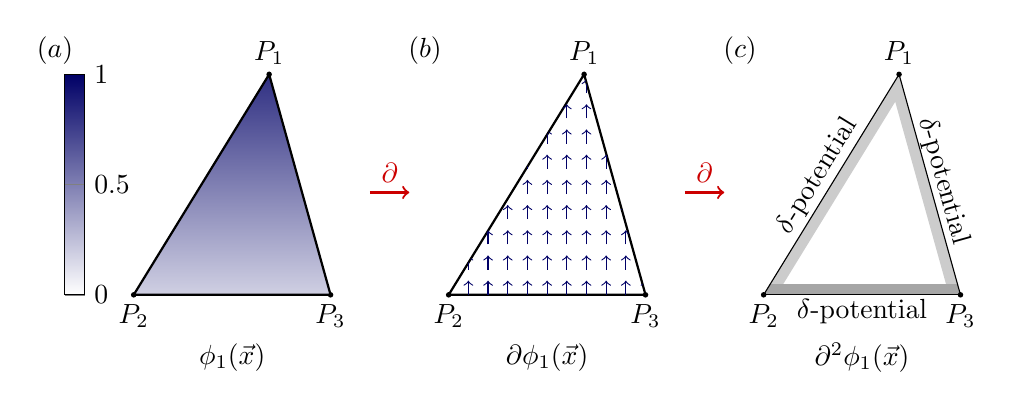
\begin{tikzpicture}
  % 在 (0,0) 处插入图片,宽度设为3cm
  %\node at (0,0) {\includegraphics[width=6.5cm]{FigSchematicFEM02.png}};
  %\node at (4,0) {\includegraphics[width=4cm]{FigSchematicFEM02.png}};

\begin{scope}[xshift=-5.3cm, yshift=0cm]
\begin{axis}[
      hide axis,
      scale only axis,
      height=\Height cm,
      width=0.25cm,
      colorbar,
      colorbar style={
        width=0.25cm,
        ytick={0,0.5,1},
        yticklabels={$0$,$0.5$, $1$},
        ylabel={},
        y label style={at={(0.5,1.05)}}
      },
      colormap={mybar}{color=(white) color=(mydarkblue)},
      point meta min=0,
      point meta max=1,
    ]
    % 只需一条虚拟数据即可生成色带
    \addplot [draw=none, samples=2] coordinates {(-3,0) (-3,1)};
  \end{axis}
  \end{scope}

%%%%%%%%%%%%%%%%%%%%%%%%%%%%%%%%%%%%%%%%%%%%%%%%%%%%%%%%%%%%%%%%%%%%%%%%%%%%%%%%%%%%%%%%%%%%%%

 \coordinate (PS) at (-4, 0);
 \coordinate (P2) at ($(0, 0) + (PS)$);
 \coordinate (P3) at ($(\Width, 0) + (PS)$);
 \coordinate (P1) at ($(\Width * 0 .688, \Height) + (PS)$);

 \node[above] at (P1) {$P_1$};
 \node[below] at (P2) {$P_2$};
 \node[below] at (P3) {$P_3$};

\fill (P1) circle (1pt);
\fill (P2) circle (1pt);
\fill (P3) circle (1pt);

\pgfdeclareverticalshading{myverticalshade}{\Height cm}{
    color(0cm)=(white);
    color(\Height cm)=(mydarkblue)
  }

  % 用该渐变填充三角形
  \shade[shading=myverticalshade]
    (P1) -- (P2) -- (P3) -- cycle;

  % 可加边框
  \draw[thick] (P1) -- (P2) -- (P3) -- cycle;

  \coordinate (E) at ($(P2)!0.5!(P3) + (0,-0.8)$);
  \node at (E) {$\phi_1(\vec{x})$};


%%%%%%%%%%%%%%%%%%%%%%%%%%%%%%%%%%%%%%%%%%%%%%%%%%%%%%%%%%%%%%%%%%%%%%%%%%%%%%%%%%%%%%%%%%%%%%%%%%%%%%%%%%%%%%%%%%%%%%%%%%%%%%%%%%%%

\coordinate (PS) at (0, 0);
 \coordinate (P2) at ($(0, 0) + (PS)$);
 \coordinate (P3) at ($(\Width, 0) + (PS)$);
 \coordinate (P1) at ($(\Width * 0 .688, \Height) + (PS)$);

  % 画三角形边界
  \draw[thick] (P1) -- (P2) -- (P3) -- cycle;

  % 画垂直向上的矢量场
 \begin{scope}
    \clip (P2) -- (P3) -- (P1) -- cycle;
    % 箭头密度参数
    \def\dx{0.25}
    \def\dy{0.32}
    \def\arrowL{0.18}
    % 扫描覆盖整个三角形的矩形网格
    \foreach \x in {0,\dx,...,4}
      \foreach \y in {0,\dy,...,3} {
        \draw[->, >=to, mydarkblue] (\x,\y) -- ++(0,\arrowL);
      }
  \end{scope}

 \node[above] at (P1) {$P_1$};
 \node[below] at (P2) {$P_2$};
 \node[below] at (P3) {$P_3$};

\fill (P1) circle (1pt);
\fill (P2) circle (1pt);
\fill (P3) circle (1pt);

\coordinate (E) at ($(P2)!0.5!(P3) + (0,-0.8)$);
  \node at (E) {$\partial\phi_1(\vec{x})$};

%%%%%%%%%%%%%%%%%%%%%%%%%%%%%%%%%%%%%%%%%%%%%%%%%%%%%%%%%%%%%%%%%%%%%%%%%%%%%%%%%%%%%%%%%%%%%%%%%%%%%%%%%%%%%%%%%%%%%%%%%%%%%%%%%%%%

\coordinate (PS) at (4, 0);
 \coordinate (P2) at ($(0, 0) + (PS)$);
 \coordinate (P3) at ($(\Width, 0) + (PS)$);
 \coordinate (P1) at ($(\Width * 0 .688, \Height) + (PS)$);

 \begin{scope}
    \clip (P2) -- (P3) -- (P1) -- cycle;
    % 箭头密度参数
   \draw[gray!40, line width=8.0] (P1) -- (P2);
\draw[gray!40, line width=8.0] (P1) -- (P3);
\draw[gray!70, line width=8.0] (P2) -- (P3);
  \end{scope}
  
 \node[above] at (P1) {$P_1$};
 \node[below] at (P2) {$P_2$};
 \node[below] at (P3) {$P_3$};

\fill (P1) circle (1pt);
\fill (P2) circle (1pt);
\fill (P3) circle (1pt);

%\coordinate (E) at ($(P2)!0.5!(P3)$);
%\node at (E) {$\delta$-potential};

\draw (P1) -- (P2) node[midway, above, sloped, yshift = -2] {$\delta$-potential};
\draw (P1) -- (P3) node[midway, above, sloped, yshift = -3] {$\delta$-potential};
\draw (P2) -- (P3) node[midway, below, sloped, yshift = 2] {$\delta$-potential};

\coordinate (E) at ($(P2)!0.5!(P3) + (0,-0.8)$);
  \node at (E) {$\partial^2\phi_1(\vec{x})$};

%%%%%%%%%%%%%%%%%%%%%%%%%%%%%%%%%%%%%%%%%%%%%%%%%%%%%%%%%%%%%%%%%%%%%%%%%%%%%%%%%%%%%%%%%%%%%%%%%%%%%%%%%%%%%%%%%%%%%%%%%%%%%%%%%%%

\node at (-5, \Height + 0.3) {$(a)$};
\node at (-0.3, \Height + 0.3) {$(b)$};
\node at (3.7, \Height + 0.3) {$(c)$};

\draw[->, >=to, thick, color = myred] (-1,1.3) -- (-0.5,1.3) 
    node[midway, above, sloped] {$\partial$};
\draw[->, >=to, thick, color = myred] (3,1.3) -- (3.5,1.3) 
    node[midway, above, sloped] {$\partial$};


  
\end{tikzpicture}
\end{document}